%
%

\pdfbookmark[1]{Вступ}{intro}
\section*{Вступ}

 
\section{Назва}


\section{Назва}


\section{Приклади оформлення окремих елементів статті}

Формули з скрізним номером: 
\begin{equation}\label{radap1725eq1}
p_n(z(\xi)) = \frac{1}{\sqrt{2\pi} v} \exp  \left(-\frac{1}{2}\Bigg(\frac{z(\xi)}{v} \Bigg)^2 \right)
\end{equation}

\begin{equation}\label{radap1725eq2}
p_{cn}(z(\xi)) = \frac{1}{\sqrt{2\pi} v} \exp  \left(-\frac{1}{2}\Bigg(\frac{z(\xi)}{v}-q \Bigg)^2 \right) 
\end{equation}

Декілька рівнянь з позначкою одним номером:
\begin{equation*}
\begin{aligned}
{K_1}\left( {x,y} \right) = {C_1}\left( {x,y} \right) + {n_1}\left( {x,y} \right),\\	
{K_2}\left( {x,y} \right) = {C_2}\left( {x,y} \right) + {n_2}\left( {x,y} \right),
\end{aligned}
\end{equation*}

%\begin{equation}
%\begin{aligned}
%
%\end{aligned}
%\end{equation}

Довгі формули слід записувати у декілька стрічок як це приведено нижче:
\begin{multline}\label{radap1345eq2}
U_{i-1}= \sum\limits_{j=0}^{i-1}\left| r_j - \sum\limits_{h=0}^{g} x_{(j-h)} \nu_h \right|^2 =\\= \sum\limits_{j=0}^{i-2}\left| r_j - \sum\limits_{h=0}^{g} x_{(j-h)} \nu_h \right|^2 +w_{i-1} =\\= U_{i-2} + w_{i-1} 
\end{multline}

Дуже довгі формули, що важко розмістити в одній колонці можна розмістити на всю сторінку як це приведено нижче:

\end{multicols} % Закриваємо розмітку на дві колонки
\begin{multline}
\upsilon({{s}_{x}},{{s}_{y}},{{s}_{z}})\!=\!\frac{\left[{{p}_{\bot }}{{J}_{1}}\left(\sqrt{s_{x}^{2}+s_{y}^{2}}{{r}_{0}}\right){{J}_{0}}({{p}_{\bot }})-\sqrt{s_{x}^{2}+s_{y}^{2}}{{r}_{0}}{{J}_{0}}\left(\sqrt{s_{x}^{2}+s_{y}^{2}}{{r}_{0}}\right){{J}_{1}}({{p}_{\bot }})\right]}{(s_{x}^{2}+s_{y}^{2})r_{0}^{2}-p_{\bot }^{2}}\frac{\omega _{z}^{*}({{s}_{z}})}{\sqrt{s_{x}^{2}+s_{y}^{2}}};  
\end{multline}
\begin{multicols}{2} % Відкриваємо нову розмітку на дві колонки 

Формули без номеру: 
$$
M\left\{ {\ln \left( {\left. \Lambda  \right|\xi } \right)} \right\} = \frac{{{{\left( {{\rm M}\left\{ {z\left( \xi  \right)} \right\}} \right)}^2}}}{{2{v^2}}}.
$$	
 
   
  

\section{ }

\subsection{Рисунки}
 
\begin{Figure}\centering%{l}{\linewidth}
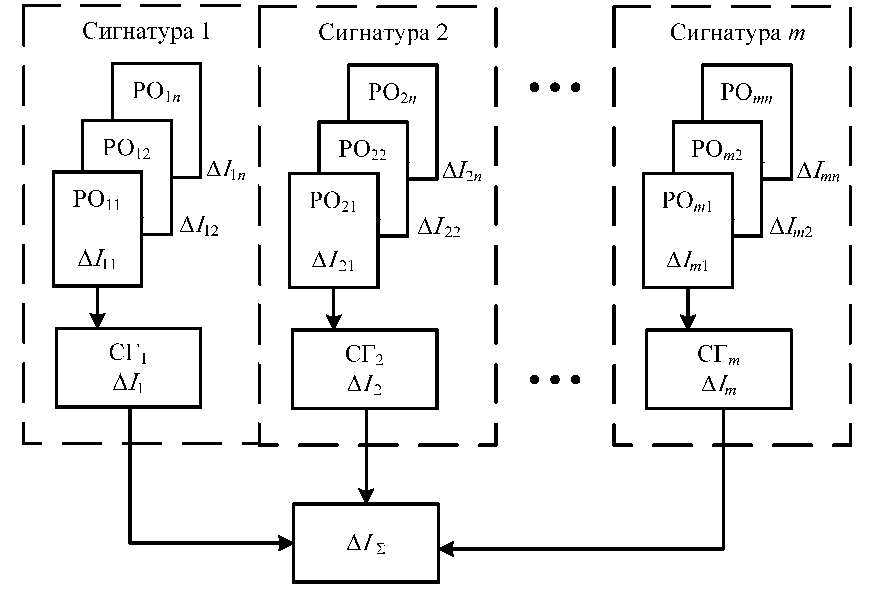
\includegraphics[width=\linewidth]{fig1}
\captionof{figure}{Графік залежності помилки визначення висот об'єктів від значення базису стереознімання}\label{radap1627fig1}
\end{Figure}
 
\begin{figure*}\centering
	%Figure 5 	
	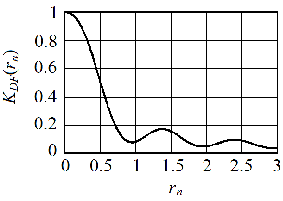
\includegraphics[width=0.4\linewidth]{fig2a}
	~~~~~
	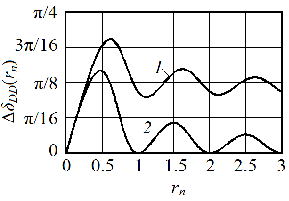
\includegraphics[width=0.4\linewidth]{fig2b}
	\begin{tabular}{p{0.49\linewidth}p{0.49\linewidth}}
		\centering (a) & \centering (b)  
	\end{tabular}	
	\captionof{figure}{Підпис до рисунку (a) $\Delta\delta_{DD}(r_n)$ (b)  $\theta = 1 $}\label{fig2}%
\end{figure*}

\subsection{Оформлення таблиць}

Таблиця в одній колонці
\begin{Table}
	\captionof{table}{Назва таблиці}
	\begin{tabularx}{\linewidth}{|l|c|c|c|c|X|}
		\hline   &   &  &  &  &  \\
		\rule{0pt}{10pt}   &   &	 &	  & &	 \\ 
		\hline 
		\rule{0pt}{10pt}  &  &   &	  &	  &  \\ 
		\hline 
		\rule{0pt}{10pt}  &   &	 &	  &	  &	 \\ 
		\hline 
		\rule{0pt}{10pt}  &   &   &	  &	  & \\ 
		\hline 
		\rule{0pt}{10pt}   &	  &  &   &	  &  \\ 
		\hline 
\end{tabularx} \label{radap1725tab1}
\end{Table}

Таблиця на дві колонки
\end{multicols}
\begin{Table}
\captionof{table}{Назва таблиці}
\begin{tabularx}{\linewidth}{|l|c|c|c|c|X|}
	\hline   &   &  &  &  &  \\
	\rule{0pt}{10pt}   &   &	 &	  & &	 \\ 
	\hline 
	\rule{0pt}{10pt}  &  &   &	  &	  &  \\ 
	\hline 
	\rule{0pt}{10pt}  &   &	 &	  &	  &	 \\ 
	\hline 
	\rule{0pt}{10pt}  &   &   &	  &	  & \\ 
	\hline 
	\rule{0pt}{10pt}   &	  &  &   &	  &  \\ 
	\hline 
\end{tabularx} \label{radap1725tab2}
\end{Table}
\begin{multicols}{2}




\pdfbookmark[1]{Висновки}{conc}
\section*{Висновки}



\pdfbookmark[1]{Перелік посилань}{lit}
\section*{Перелік посилань}

\href{http://radap.kpi.ua/radiotechnique/citing}{Правила оформлення посилань}

\pdfbookmark[1]{References}{translit}
\renewcommand{\refname}{References}

\begin{thebibliography}{99}\footnotesize 
	
	\bibitem{radap1725ref1} Omelianenko M., Romanenko T. (2020). E-plane Stepped-Impedance Bandpass Filter with Wide Stopband. \href{https://ieeexplore.ieee.org/abstract/document/9088888}{\textit{2020 IEEE 40th International Conference on Electronics and Nanotechnology (ELNANO)}}, pp. 838-841, doi: 10.1109/ELNANO50318.2020.9088888.
	
	\bibitem{radap1725ref2}	 
	
	\bibitem{radap1725ref3}	 
	
	\bibitem{radap1725ref4}	 
	
	\bibitem{radap1725ref5}	 
	
	\bibitem{radap1725ref6}	 
	
	\bibitem{radap1725ref7}	 
	
	\bibitem{radap1725ref8}	 
	
	\bibitem{radap1725ref9}	 
	
	\bibitem{radap1725ref10}
	
	\bibitem{radap1725ref11} 
	
	\bibitem{radap1725ref12}	 
	
	\bibitem{radap1725ref13}	 
	
	\bibitem{radap1725ref14}	 
	
	\bibitem{radap1725ref15}	 	 
	
\end{thebibliography}